\subsection{函子 TS}

设 M, N 为 A-模，u 为 M 到 N 的同态；显然 \(\mathbf{T}(u)(\mathbf{TS}(\mathbf{M})) \subset \mathbf{TS}(\mathbf{N})\) 。从 \(\mathbf{TS}(\mathbf{M})\) 到 \(\mathbf{TS}(\mathbf{N})\) 的、由 \(\mathbf{T}(u)\) 得到的映射用 \(\mathbf{TS}(u)\) 表示。容易验证这是分次代数的一个保单位同态，并且我们有 \(\mathbf{TS}(u)\left(\gamma_{p}(x)\right) = \gamma_{p}(u(x))\) （对所有 \(x \in M\) 及每个整数 \(p \geqslant 0\) ）。若 \(v : N \to P\) 是 A-模的一个同态，我们有

\[
\mathbf {T S} (v \circ u) = \mathbf {T S} (v) \circ \mathbf {T S} (u).
\]

根据TS(u)的定义，图表

\pandocbounded{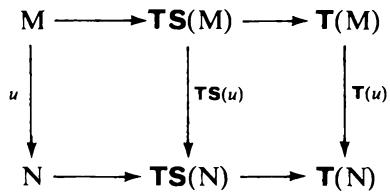
\includegraphics[keepaspectratio]{images/part001_53632150.jpg}}

是交换的，其中水平箭头表示典范单射。

若 M 是 N 的一个直因子，且 \(i: M \rightarrow N\) 是典范单射，则 \(\mathbf{TS}(i)\) 是从 \(\mathbf{TS}(\mathbf{M})\) 到 \(\mathbf{TS}(\mathbf{N})\) 的一个直因子 R 上的单同态，我们通常借此把 \(\mathbf{TS}(\mathbf{M})\) 与 R 等同。其证明与张量代数的证明相同（III，第 487 页）。

假设 M 是一个子模族 \((\mathbf{M}_{\lambda})_{\lambda \in L}\) 的直和。典范单射 \(\mathbf{TS}(\mathbf{M}_{\lambda}) \to \mathbf{TS}(\mathbf{M})\) 定义了分次代数的一个保单位同态 h，称为典范同态：

\[
\underset {\lambda \in L} {\otimes} \mathbf {T S} \left(\mathrm{M} _ {\lambda}\right)\rightarrow \mathbf {T S} (\mathrm{M}).
\]

设 \(\lambda_1, \lambda_2, \ldots, \lambda_n\) 是 \(L\) 中两两不同的元素，并令 \(x_1 \in M_{\lambda_1}, \ldots, x_n \in M_{\lambda_n}\) 。根据 IV 第 45 页命题 3 (ii)，我们有

\[
h \left(\sum_ {p _ {1} + \dots + p _ {n} = p} \gamma_ {p _ {1}} (x _ {1}) \otimes \dots \otimes \gamma_ {p _ {n}} (x _ {n})\right) = \gamma_ {p} (x _ {1} + \dots + x _ {n}).\tag{8}
\]

设 N 是一个 A-模，它是子模族 \((\mathbf{N}_{\lambda})_{\lambda \in L}\) 的直和。对于每一个 \(\lambda \in L\) ，令 \(u_{\lambda}\) 是从 \(M_{\lambda}\) 到 \(N_{\lambda}\) 的一个同态。设 u 是由 \(u_{\lambda}\) 定义的从 M 到 N 的同态。则图表

\[
\begin{array}{c} \otimes \mathsf {T S} (\mathrm{M} _ {\lambda}) \xrightarrow {h} \mathsf {T S} (\mathrm{M}) \\ \otimes \mathsf {T S} (u _ {\lambda}) \Bigg | _ {\downarrow} \qquad \qquad \qquad \qquad \qquad \qquad \qquad \qquad \qquad \qquad \qquad \qquad \qquad \qquad \qquad \qquad \qquad \qquad \qquad \qquad \qquad \qquad \qquad \qquad \qquad \qquad \qquad \qquad \qquad \qquad \qquad \qquad \qquad \qquad \\ \otimes \mathsf {T S} (\mathrm{N} _ {\lambda}) \xrightarrow {h ^ {\prime}} \mathsf {T S} (\mathrm{N}) \end{array}
\]

可交换，其中 h 和 \(h'\) 是典范同态。因为若 \(z \in TS(M_{\lambda})\) ，且 \(i_{\lambda}\) （相应地 \(j_{\lambda}\) ）表示 \(M_{\lambda}\) 到 M 的典范单射（相应地，\(N_{\lambda}\) 到 N 的典范单射），则我们有

\[
\begin{array}{r l} \mathbf {T S} (u) (h (z)) & = \mathbf {T S} (u) \circ \mathbf {T S} (i _ {\lambda}) (z) = \mathbf {T S} (u \circ i _ {\lambda}) (z) = \\ & = \mathbf {T S} (j _ {\lambda} \circ u _ {\lambda}) (z) = \mathbf {T S} (j _ {\lambda}) \circ \mathbf {T S} (u _ {\lambda}) (z) = h ^ {\prime} (\mathbf {T S} (u _ {\lambda}) (z)). \end{array}
\]

命题 6. --- 设 M 是一个 A-模，它是子模族 \((\mathbf{M}_{\lambda})_{\lambda \in L}\) 的直和。若每个 \(M_{\lambda}\) 是自由模，则从 \(\otimes \mathbf{TS}(\mathbf{M}_{\lambda})\) 到 \(\mathbf{TS}(\mathbf{M})\) 的典范同态是一个同构。

设 \((e_{i,\lambda})_{i\in I_{\lambda}}\) 是 \(\mathbf{M}_{\lambda}\) 的一组基。对于 \(\nu \in \mathbf{N}^{(I_{\lambda})}\) ，令 \(e_{\nu ,\lambda} = \prod_{i\in I_{\lambda}}\gamma_{\nu (i)}(e_{i,\lambda})\) 。这些 \(e_{\nu ,\lambda}\) （\(\nu \in \mathbf{N}^{(I_{\lambda})}\) ）构成 \(\mathbf{TS}(\mathbf{M}_{\lambda})\) 的一组基（IV，第 47 页，命题 4 (i)），且 \(e_{0,\lambda}\) 是 \(\mathbf{TS}(\mathbf{M}_{\lambda})\) 的单位元。因此这些元素

\[
\bigotimes_ {\lambda \in L} e _ {\nu_ {\lambda}, \lambda}\tag{9}
\]

，其中 \(\nu_{\lambda} \in \mathbf{N}^{(I_{\lambda})}\) 且除有限多个指标外 \(\nu_{\lambda} = 0\) ，构成 \(\otimes_{\lambda} \mathbf{TS}(M_{\lambda})\) 的一组基。命题中的典范同态把元素 (9) 映为 \(\prod_{\lambda \in L} e_{\nu_{\lambda,\lambda}}\) 。如果我们用 \((e_i)_{i \in I}\) 表示这些族 \((e_{i,\lambda})_{i \in I_{\lambda}}\) 的不交并，则上述元素恰好是 \(\prod_{i \in I} \gamma_{\nu(i)}(e_i)\) （其中 \(\nu \in \mathbf{N}^{(I)}\) ），因此它们构成 \(\mathbf{TS}(M)\) 的一组基。这就证明了该命题。

在命题 6 的条件下，逆同构 \(\mathbf{TS}(\mathbf{M}) \to \otimes_{\lambda} \mathbf{TS}(\mathbf{M}_{\lambda})\) 也称为典范的。通常把 \(\mathbf{TS}(\mathbf{M})\) 与

\(\otimes_{\lambda} \mathbf{TS}(M_{\lambda})\) 借助此同构等同起来。应当注意，若 \(z \in \mathbf{TS}(M_{\lambda})\)

\pandocbounded{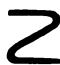
\includegraphics[keepaspectratio]{images/part001_3a9079a2.jpg}}

且 \(z' \in \mathbf{TS}(M_{\mu})\) （\(\lambda \neq \mu\) ），那么我们由此被引导用 \(z \otimes z'\) 表示的 TS(M) 的元素并不是 z 与 \(z'\) 在 T(M) 中的张量积，而是 z 与 \(z'\) 的对称积。

命题 7. --- 设 M 为一个 A-模，u 为映射 \((x, y) \mapsto x + y\) （从 \(M \oplus M\) 到 M 中），且 f 为复合映射

\[
\mathbf {T S} (\mathrm{M}) \otimes \mathbf {T S} (\mathrm{M}) \xrightarrow {h} \mathbf {T S} (\mathrm{M} \oplus \mathrm{M}) \xrightarrow {\mathbf {T S} (u)} \mathbf {T S} (\mathrm{M})
\]

，其中 \(h\) 是典范同态。若 \(z, z' \in \mathbf{TS}(\mathbf{M})\) ，则 \(f(z \otimes z') = zz'\) 。

设 \(i\) 为映射 \(x \mapsto (x, 0)\) （从 M 到 M ⊕ M 中的）。我们有 \(u \circ i = \mathrm{Id}_{\mathbf{M}}\) ，因此 \(\mathbf{TS}(u) \circ \mathbf{TS}(i) = \mathrm{Id}_{\mathbf{TS}(\mathbf{M})}\) ；因此

\[
f (z \otimes 1) = \mathbf {T S} (u) (h (z \otimes 1)) = \mathbf {T S} (u) (\mathbf {T S} (i) (z)) = z.
\]

同样地 \(f(1 \otimes z') = z'\) ，从而 \(f(z \otimes z') = f(z \otimes 1)\) \(f(1 \otimes z') = zz'\) 。

